%===================================== CHAP 2 =================================

\chapter{Background Theory}

\section{Artificial Neural Networks}

\textit{This was missing in the specialization project. Need to cover all concepts used later in the report. This includes all different layers of a neural network. The layers (dropout, pooling, etc) could perhaps be a separate section after this one.}

\subsection{The Neuron}

Artificial Neural Networks (ANNs) are inspired by the structure and behavior of a biological brain, but they are generally not intended to be realistic models. A neural network consist of interconnected nodes referred to as units. These correspond to a biological neuron, the basic computational unit of the brain, structured as illustrated in \textbf{Fig. \ref{fig1}}. The connections between the units in an  corresponds to a biological neuron's dendrites, which provide input signals, and its single axon, which produces output signals and is connected to other neurons. \\

\begin{figure}
    \begin{minipage}{0.5\textwidth}
        \centering
            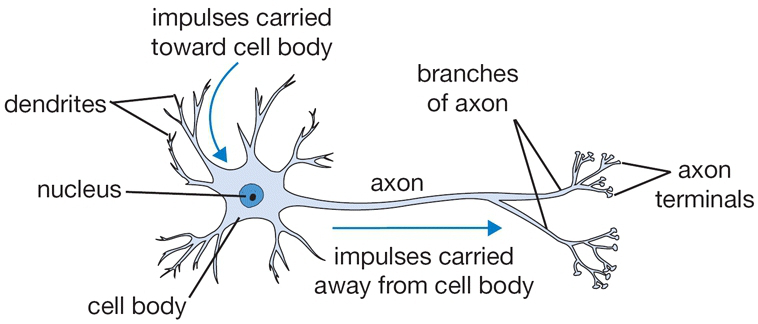
\includegraphics[width=1\textwidth]{fig/neuron}
            \caption{Biological neuron\cite{cs231n_part1}}
            \label{fig1}
    \end{minipage}
    \begin{minipage}{0.4\textwidth}
        \centering
            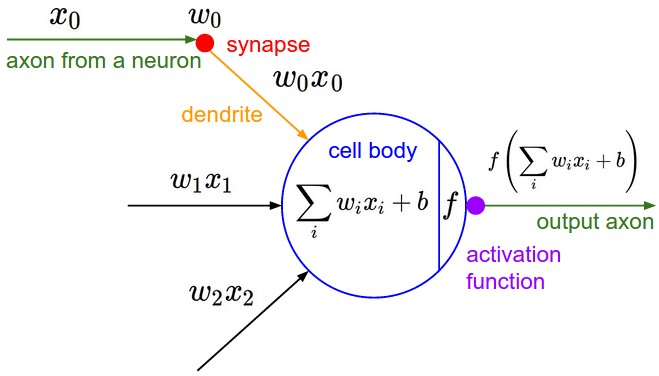
\includegraphics[width=1\textwidth]{fig/neuron_model}
            \caption{Mathematical model of a neuron\cite{cs231n_part1}}
            \label{fig2}
    \end{minipage}
\end{figure}

\noindent To simulate these signals, an ANN uses a mathematical model as illustrated in \textbf{Fig. \ref{fig2}}, where the signal is multiplied by the weight of a connection. The weight of a specific connection control how much the unit on one end influences the unit on the other end. The sum of all input signals are computed at the cell body of the unit. If this sum is above a certain threshold, the unit fires an output signal determined by its activation function by performing a specific mathematical operation on the sum. The idea of an ANN is that it can approximate any continuous function, and that it has the possibility of learning. The weights of a model can be learned by training the model on a set of input and output values, a task which is called supervised learning. There are two other kinds of learning: unsupervised and reinforcement learning, but we will not cover these.\\

\noindent An ANN is usually organized in layers, where a layer consists of one or more units. The first layer is called the input layer, while the last layer is called the output layer. Any layers in between are called hidden layers. The simplest form of an ANN is the single-layer perceptron, which consists of only one layer of output nodes. This network can only learn linearly separable patterns. To allow for learning complex patterns, more layers need to be added. As layers are added, the depth of the network increases. This is why we refer to the use of multi-layer perceptrons (MLPs) as "deep learning". \\

\noindent There are several different classes and types of ANNs. We will only describe the feedforward neural network, which is the original version, and thus we will use the term ANN when referring to such a network. In this kind of network, all connections are from one layer to the next layer, and there are no cycles or connections between units in the same layer. A network with cycles is called a recurrent neural network (RNN).

\subsection{Optimization}

The goal of an ANN is to find a function that solves a specific problem, more specifically that finds an optimal solution. The definition of this optimal solution is that given a cost function, there are no other solution with less of a cost. The cost function is in that sense a measure of how far away a solution is from an optimal solution. The goal of the learning process is thus to find a a function with the smallest possible cost. In supervised learning, this means to find the function that best maps the input to the output. The cost will then be the mismatch between such a mapping and the example data, and is often calculated using the mean squared error (MSE), defined as the average of the squares of the errors:
\begin{equation}
    MSE = \frac{1}{n}\sum_{i=1}^{n}(\hat{Y}_i - Y_i)^2
\end{equation}

\noindent To optimize the cost, we can use an algorithm called gradient descent, which minimizes any function iteratively. The process is a repeated loop of evaluating the gradient of the cost function, and then updating the weights based on this gradient. There are a number of different algorithms to optimize this process, and we will following describe the ones commonly used.

\subsubsection{Stochastic Gradient Descent}

\subsubsection{RMSprop}
\subsubsection{Adagrad}
\subsubsection{Adadelta}

\begin{itemize}
    \item SGD
    \item RMSprop
    \item Adagrad
    \item Adadelta
    \item Adam
    \item Adamax
    \item basically all optimizers keras provide, or only the ones we actually end up using
\end{itemize}

\begin{itemize}
    \item backpropagation
\end{itemize}

\subsection{The Activation Function}

\noindent There are a great variety of activation functions in use, but we will only briefly describe those most commonly used and thus considered in our implementation. The mathematical function of these are plotted in \textbf{Fig. \ref{activationfuncs}}. For further details we refer the reader to the Stanford CS class on convolutional neural networks\cite{cs231n_part1}. The common behaviour of all activation functions is that they define the output of a unit given a set of inputs. \\
\begin{figure}[H]
    \begin{minipage}{0.3\textwidth}
        \begin{tikzpicture}
            \begin{axis}[
                title = {Sigmoid function},
                axis lines = center,
                xtick={-10, -5, 5, 10},
                ytick={0, 0.2, 0.4, 0.6, 0.8, 1.0},
            ]
            \addplot [
                domain=-10:10,
                samples=100,
                color=blue,
            ]
            {1 / (1 + e^-x)};
            \end{axis}
        \end{tikzpicture}
    \end{minipage}
    \begin{minipage}{0.3\textwidth}
        \begin{tikzpicture}
            \begin{axis}[
                title = {Tanh function},
                axis lines = center,
                xtick={-10, -5, 5, 10},
                ytick={-1.0, -0.5, 0, 0.5, 1.0},
            ]
            \addplot [
                domain=-10:10,
                samples=100,
                color=blue,
            ]
            {(2 * (1 / (1 + e^-(2*x)))) - 1};
            \end{axis}
        \end{tikzpicture}
    \end{minipage}
    \begin{minipage}{0.3\textwidth}
        \begin{tikzpicture}
            \begin{axis}[
                title = {ReLU function},
                axis lines = center,
                xtick={-10, -5, 5, 10},
                ytick={2, 4, 6, 8, 1.0},
            ]
            \addplot [
                domain=-10:10,
                samples=100,
                color=blue,
            ]
            {max(0, x)};
            \end{axis}
        \end{tikzpicture}
    \end{minipage}
    \caption{The most commonly used activation functions}
    \label{activationfuncs}
\end{figure}

\subsubsection{Sigmoid}

The sigmoid activation function is mathematically defined as $\sigma(x) = 1/(1 + e^{-x})$. The function takes a number as input, and outputs a number within a continuous range from 0 to 1. The sigmoid function has previously been used a lot, but because of its drawbacks, other activations functions tend to be preferred nowadays. The first drawback is that the outputs are not centered around zero, which can cause undesirable behaviour during gradient descent. A bigger drawback is that the activation saturates, meaning that the unit outputs mostly 0 and 1 instead of anything in between, and thus the gradient at these regions is very low. If the gradient falls to zero, the weights will not be updated through gradient descent, and so the network will stop learning.

\subsubsection{Tanh}

The tanh activation function is a scaled version of the sigmoid function. Its mathematical function is $tanh(x) = 2\sigma(2x) - 1$. The scaling causes the tanh function to output numbers within the range of -1 and 1. This makes the output zero-centered, thus avoiding the first drawback of the sigmoid function. Even though the tanh function still stuffers from saturation, it is preferred to the sigmoid function.

\subsubsection{ReLU}

The Rectified Linear Unit (ReLU) activation has the mathematical function $f(x) = max(0,x)$. This means that it is very close to linear; thresholding the input at zero, but keeping any value above. It has become very popular, and is in general the activation function of choice. It is non-saturating, and has been found to speed up the convergence of stochastic gradient descent. The computation of the function is also very inexpensive compared to the sigmoid and tanh function. The only problem with the ReLU function is the possibility of "dead" units, meaning that they will never activate. Generally, lowering the learning rate can prevent this, but there have also been several attempts to fix this issue, for instance using so called PReLU or Maxout units.

\subsection{Architecture}

\begin{itemize}
    \item Input and output layers
    \item Fully-connected layer
    \item Hidden layers
    \item Deep models
    \item Convolutional layer
    \item Dropout layer
    \item Pooling
\end{itemize}

\section{Convolutional Networks}

\textit{More in-depth than covered in the specialization project. \\
What exactly is the convolutional operation? Convolutional layer (local connections and weight sharing) vs normal layer.}

\section{Residual Networks}

\section{Face Recognition}

\textit{Can probably use a lot from the specialization project here.}

\section{Facial Expression}

\textit{Here as well.}

\section{Visualization}

\textit{Describe all the different techniques, perhaps in more detail. \\
Possibly even implementation level.}

\cleardoublepage